\chapter{Úvod}
%% Úvod charakterizující kontext zadání, případně motivace.

%% Výsledná struktura vaší práce a názvy a rozsahy jednotlivých kapitol se samozřejmě budou lišit podle typu práce a podle konkrétní povahy zpracovávaného tématu. Níže uvedená struktura práce odpovídá \textit{práci implementační}, viz \cite{infodp} respektive \cite{infobp}.

Vymezení práce je graficky znázorněno na obrázku \ref{work_scope}.

\begin{figure}[h!]
\centering
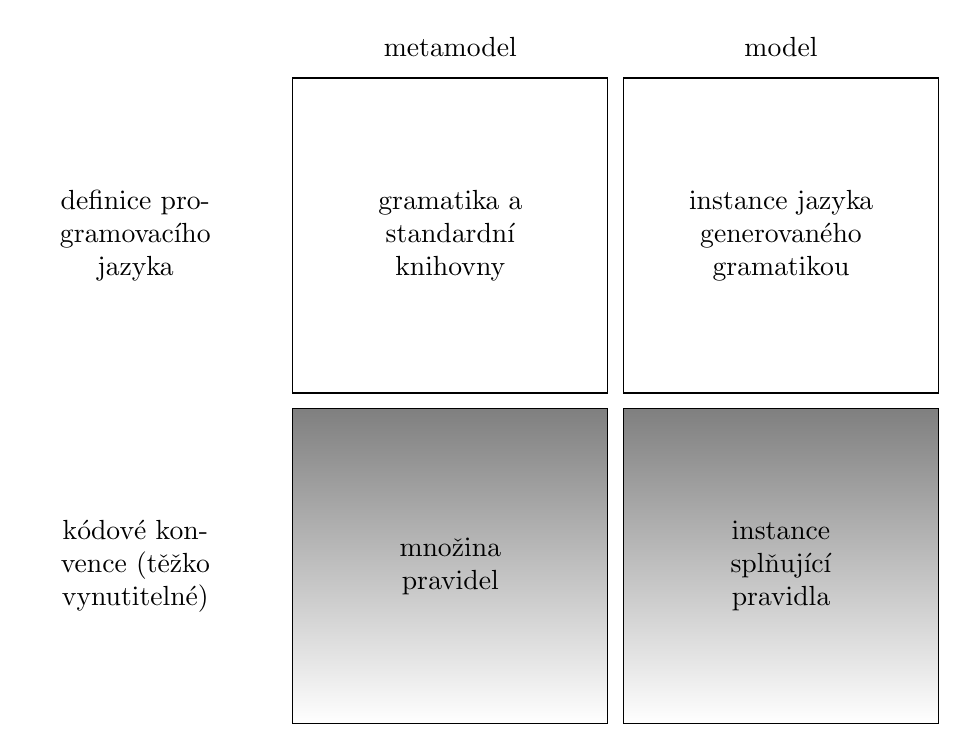
\begin{tikzpicture}
\shadedraw  (0,0) rectangle (4,4);
\shadedraw  (4.2,0) rectangle (8.2,4);
\draw  (0,4.2) rectangle (4.0,8.2);
\draw  (4.2,4.2) rectangle (8.2,8.2);

\draw  (2,2) node[text width=2.5cm, text centered] {množina pravidel};
\draw  (6.2,2) node[text width=2.5cm, text centered] {instance splňující pravidla};
\draw  (2,6.2) node[text width=2.5cm, text centered] {gramatika a standardní knihovny};
\draw  (6.2,6.2) node[text width=2.5cm, text centered] {instance jazyka generovaného gramatikou};

\draw (-2,2) node[text width=2.5cm, text centered] {kódové konvence (těžko vynutitelné)};
\draw (-2,6.2) node[text width=2.5cm, text centered] {definice programovacího jazyka};

\draw (2,8.6) node[text width=2.5cm, text centered] {metamodel};
\draw (6.2,8.6) node[text width=2.5cm, text centered] {model};
\end{tikzpicture}
\caption{Grafické znázornění zařazení práce.\label{work_scope}}
\end{figure}
